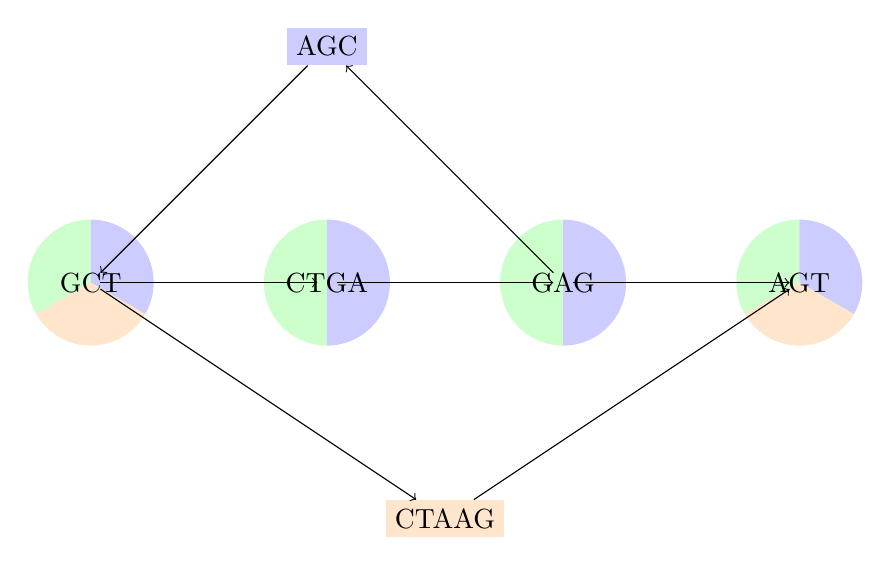
\begin{tikzpicture}[scale=1.5]
    % Define the size of the pic circles (note: pic and nodes are not the same)
    \def\a{1.6}
    % Style definitions for each row
    \tikzset{
        % one color
        one color/.style={fill=#1},
        % two colors
        pics/two colors/.style args=
        {#1|#2|label=#3}{code={%
            \fill[#1] (0,\a/2) arc(90:270:\a/2)--cycle;
            \fill[#2] (0,\a/2) arc(90:-90:\a/2)--cycle;
            \path (0,0) node[label={center:#3}] () {};
        }},
        % three colors
        pics/three colors/.style args=
        {#1|#2|#3|label=#4}{code={%
            \fill[#1] (0,\a/2) arc(90:210:\a/2)--(0,0)--cycle;
            \fill[#2] (0,\a/2) arc(90:-30:\a/2)--(0,0)--cycle;
            \fill[#3] (210:\a/2) arc(210:330:\a/2)--(0,0)--cycle;
            \path (0,0) node[label={center:#4}] () {};
        }}
    }
    % First row of nodes
    \node[one color=blue!20] (A1) at (2, 2) {AGC};

    % Second row of nodes
    \pic (B1) at (0, 0) {three colors={green!20|blue!20|orange!20|label=GCT}};
    \pic (B2) at (2, 0) {two colors={green!20|blue!20|label=CTGA}};
    \pic (B3) at (4, 0) {two colors={green!20|blue!20|label=GAG}};
    \pic (B4) at (6, 0) {three colors={green!20|blue!20|orange!20|label=AGT}};

    % Third row of nodes
    \node[one color=orange!20] (C1) at (3, -2) {CTAAG};

    % Edges between nodes
    \draw[->] (B1) -- (B2);
    \draw[->] (B2) -- (B3);
    \draw[->] (B3) -- (B4);

    \draw[->] (B1) -- (C1);
    \draw[->] (C1) -- (B4);

    \draw[<-] (B1) -- (A1);
    \draw[<-] (A1) -- (B3);
\end{tikzpicture}